\documentclass[]{article}
\usepackage{lmodern}
\usepackage{amssymb,amsmath}
\usepackage{ifxetex,ifluatex}
\usepackage{fixltx2e} % provides \textsubscript
\ifnum 0\ifxetex 1\fi\ifluatex 1\fi=0 % if pdftex
  \usepackage[T1]{fontenc}
  \usepackage[utf8]{inputenc}
\else % if luatex or xelatex
  \ifxetex
    \usepackage{mathspec}
  \else
    \usepackage{fontspec}
  \fi
  \defaultfontfeatures{Ligatures=TeX,Scale=MatchLowercase}
\fi
% use upquote if available, for straight quotes in verbatim environments
\IfFileExists{upquote.sty}{\usepackage{upquote}}{}
% use microtype if available
\IfFileExists{microtype.sty}{%
\usepackage{microtype}
\UseMicrotypeSet[protrusion]{basicmath} % disable protrusion for tt fonts
}{}
\usepackage[margin=1in]{geometry}
\usepackage{hyperref}
\hypersetup{unicode=true,
            pdftitle={Data Science Project 1},
            pdfauthor={Emily Mitchell, Alesia Andringa, Sydney Singleton},
            pdfborder={0 0 0},
            breaklinks=true}
\urlstyle{same}  % don't use monospace font for urls
\usepackage{graphicx,grffile}
\makeatletter
\def\maxwidth{\ifdim\Gin@nat@width>\linewidth\linewidth\else\Gin@nat@width\fi}
\def\maxheight{\ifdim\Gin@nat@height>\textheight\textheight\else\Gin@nat@height\fi}
\makeatother
% Scale images if necessary, so that they will not overflow the page
% margins by default, and it is still possible to overwrite the defaults
% using explicit options in \includegraphics[width, height, ...]{}
\setkeys{Gin}{width=\maxwidth,height=\maxheight,keepaspectratio}
\IfFileExists{parskip.sty}{%
\usepackage{parskip}
}{% else
\setlength{\parindent}{0pt}
\setlength{\parskip}{6pt plus 2pt minus 1pt}
}
\setlength{\emergencystretch}{3em}  % prevent overfull lines
\providecommand{\tightlist}{%
  \setlength{\itemsep}{0pt}\setlength{\parskip}{0pt}}
\setcounter{secnumdepth}{0}
% Redefines (sub)paragraphs to behave more like sections
\ifx\paragraph\undefined\else
\let\oldparagraph\paragraph
\renewcommand{\paragraph}[1]{\oldparagraph{#1}\mbox{}}
\fi
\ifx\subparagraph\undefined\else
\let\oldsubparagraph\subparagraph
\renewcommand{\subparagraph}[1]{\oldsubparagraph{#1}\mbox{}}
\fi

%%% Use protect on footnotes to avoid problems with footnotes in titles
\let\rmarkdownfootnote\footnote%
\def\footnote{\protect\rmarkdownfootnote}

%%% Change title format to be more compact
\usepackage{titling}

% Create subtitle command for use in maketitle
\newcommand{\subtitle}[1]{
  \posttitle{
    \begin{center}\large#1\end{center}
    }
}

\setlength{\droptitle}{-2em}
  \title{Data Science Project 1}
  \pretitle{\vspace{\droptitle}\centering\huge}
  \posttitle{\par}
  \author{Emily Mitchell, Alesia Andringa, Sydney Singleton}
  \preauthor{\centering\large\emph}
  \postauthor{\par}
  \predate{\centering\large\emph}
  \postdate{\par}
  \date{Updated: Sunday, August 19, 2018 @ 22:01:46}


\begin{document}
\maketitle

\paragraph{DATA FILES USED}\label{data-files-used}

\begin{itemize}
\item
  \href{ftp://aftp.cmdl.noaa.gov/products/trends/co2/co2_annmean_mlo.txt}{Source
  and description of MLCO2annual dataset}
\item
  \href{https://raw.githubusercontent.com/STAT-JET-ASU/DataScience1/master/Projects/MLCO2annual.csv}{MLC02annual
  dataset} (comma delimited text file)
\item
  \href{ftp://aftp.cmdl.noaa.gov/products/trends/co2/co2_mm_mlo.txt}{Source
  and description of MLCO2monthly dataset}
\item
  \href{https://raw.githubusercontent.com/STAT-JET-ASU/DataScience1/master/Projects/MLCO2monthly.csv}{MLCO2monthly
  dataset} (comma delimited text file)
\item
  \href{ftp://aftp.cmdl.noaa.gov/products/trends/co2/co2_weekly_mlo.txt}{Source
  and description of MLCO2weekly dataset}
\item
  \href{https://raw.githubusercontent.com/STAT-JET-ASU/DataScience1/master/Projects/MLCO2weekly.csv}{MLCO2weekly
  dataset} (comma delimited text file)
\item
  \href{https://www.esrl.noaa.gov/gmd/ccgg/trends/gr.html}{Source and
  description of MLCO2growth dataset}
\item
  \href{https://raw.githubusercontent.com/STAT-JET-ASU/DataScience1/master/Projects/MLCO2growth.csv}{MLCO2growth
  dataset} (comma delimited text file)
\end{itemize}

\paragraph{DIRECTIONS}\label{directions}

Use only the three datasets provided. In some cases, you will have to
create new variables or perform your own calculations / transformations.
When replicating graphs, you do not have to include the round NOAA and
Scripps badges or the March 2018 date stamps.

\begin{itemize}
\item
  Replicate the content of the graph shown on
  \href{https://www.esrl.noaa.gov/gmd/ccgg/trends/index.html}{this
  page}.
\item
  Replicate the content of the graph shown on
  \href{https://www.esrl.noaa.gov/gmd/ccgg/trends/full.html}{this page}.
\item
  Replicate the content of the graph shown on
  \href{https://www.esrl.noaa.gov/gmd/ccgg/trends/gr.html}{this page}.
\item
  Using the monthly data, create side-by-side boxplots of CO2 by decade.
  Exclude the 1950s (1959 and before) and 2010s (2010 and after) because
  the data for those decades is incomplete.
\item
  Use the multiplot function from the Rmisc package to create a display
  for the 21st century that includes four stacked plots. Exclude the
  incomplete 2018 data.

  \begin{itemize}
  \tightlist
  \item
    barplot of mean CO2 for each year with error bars showing
    uncertainty (using annual data)
  \item
    side-by-side boxplots of CO2 by year (using weekly data)
  \item
    side-by-side boxplots of adjusted CO2 by year (using monthly data)
  \item
    a time series plot showing the change in CO2 for one year, 10 years,
    and since 1800 (using weekly data)
  \end{itemize}
\end{itemize}

\paragraph{RESULTING GRAPHS}\label{resulting-graphs}

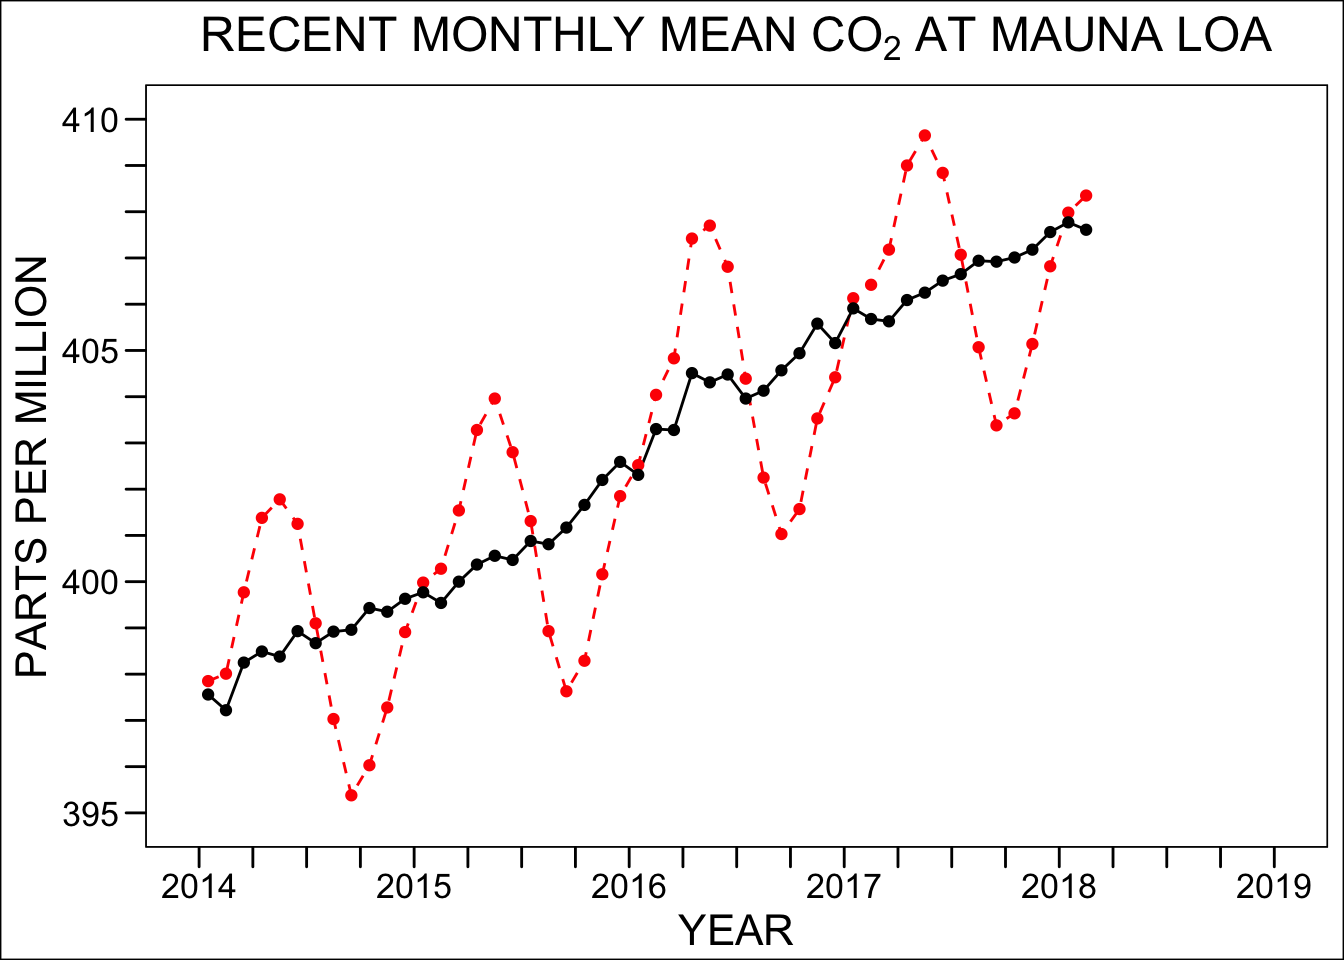
\includegraphics{Project01_files/figure-latex/unnamed-chunk-2-1.pdf}

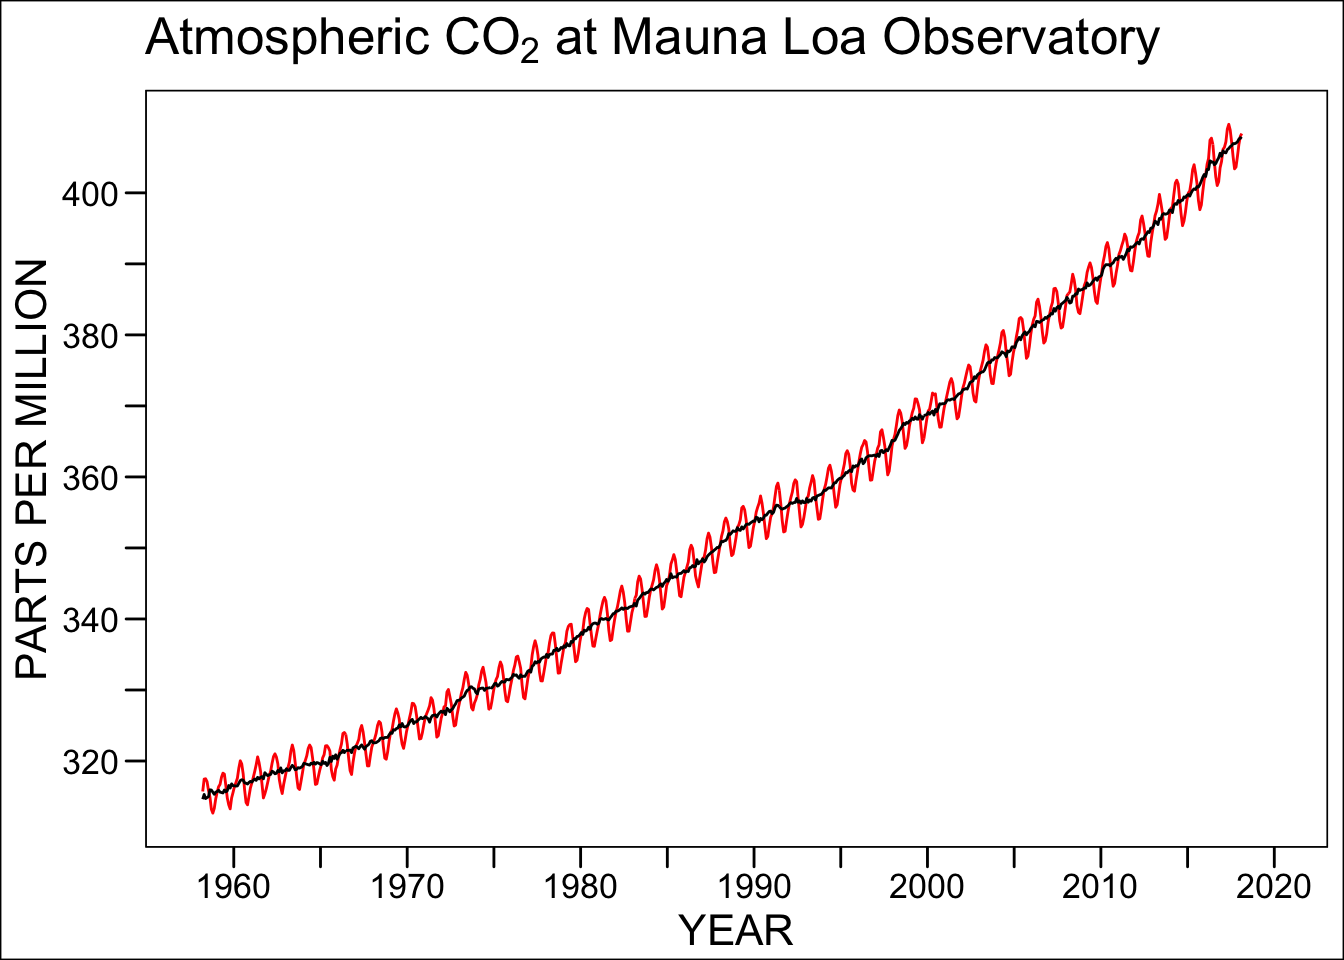
\includegraphics{Project01_files/figure-latex/unnamed-chunk-3-1.pdf}

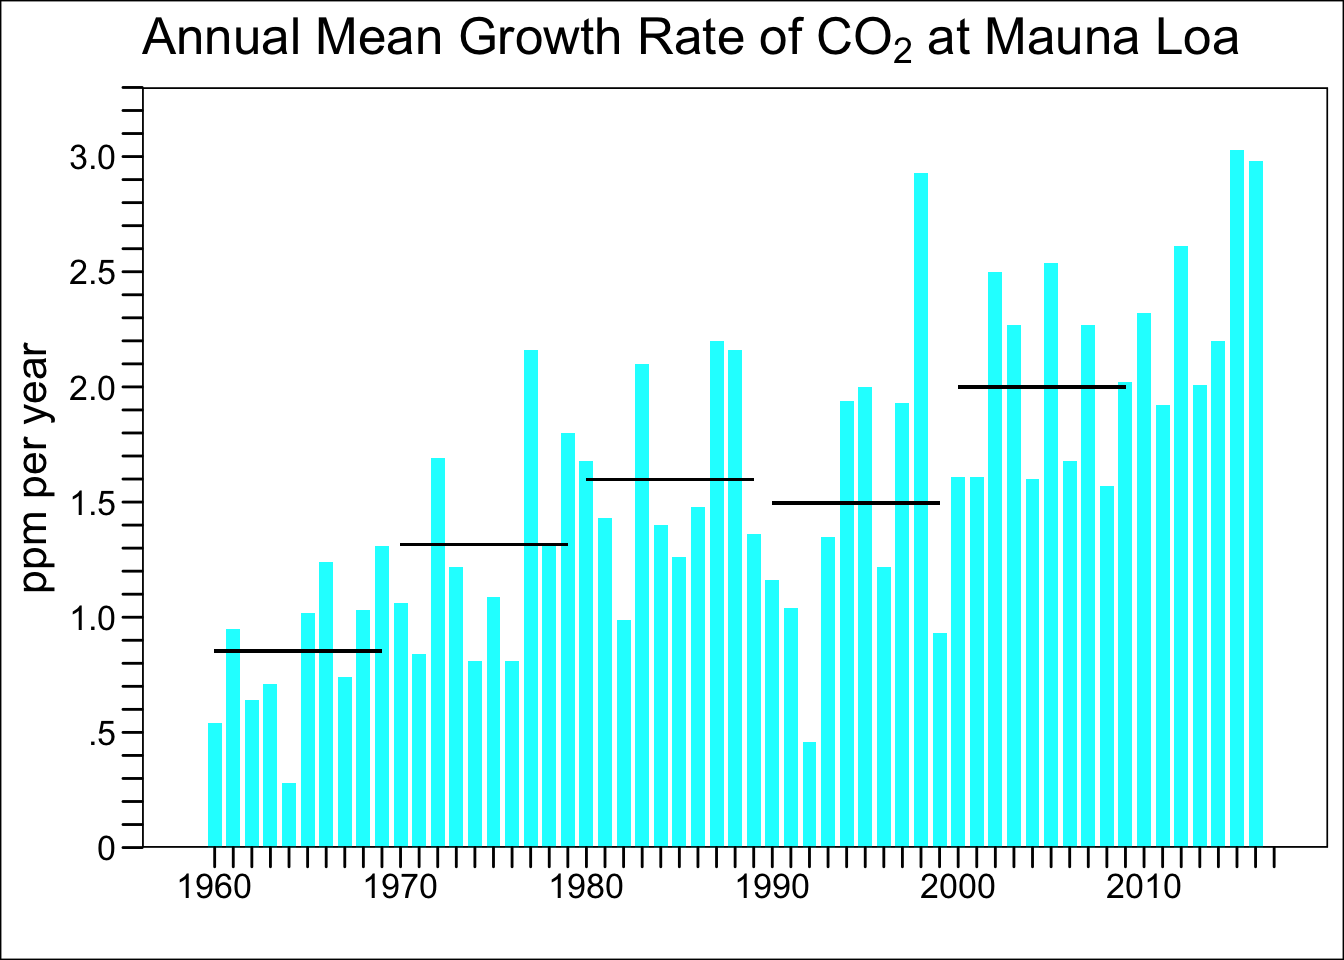
\includegraphics{Project01_files/figure-latex/unnamed-chunk-4-1.pdf}

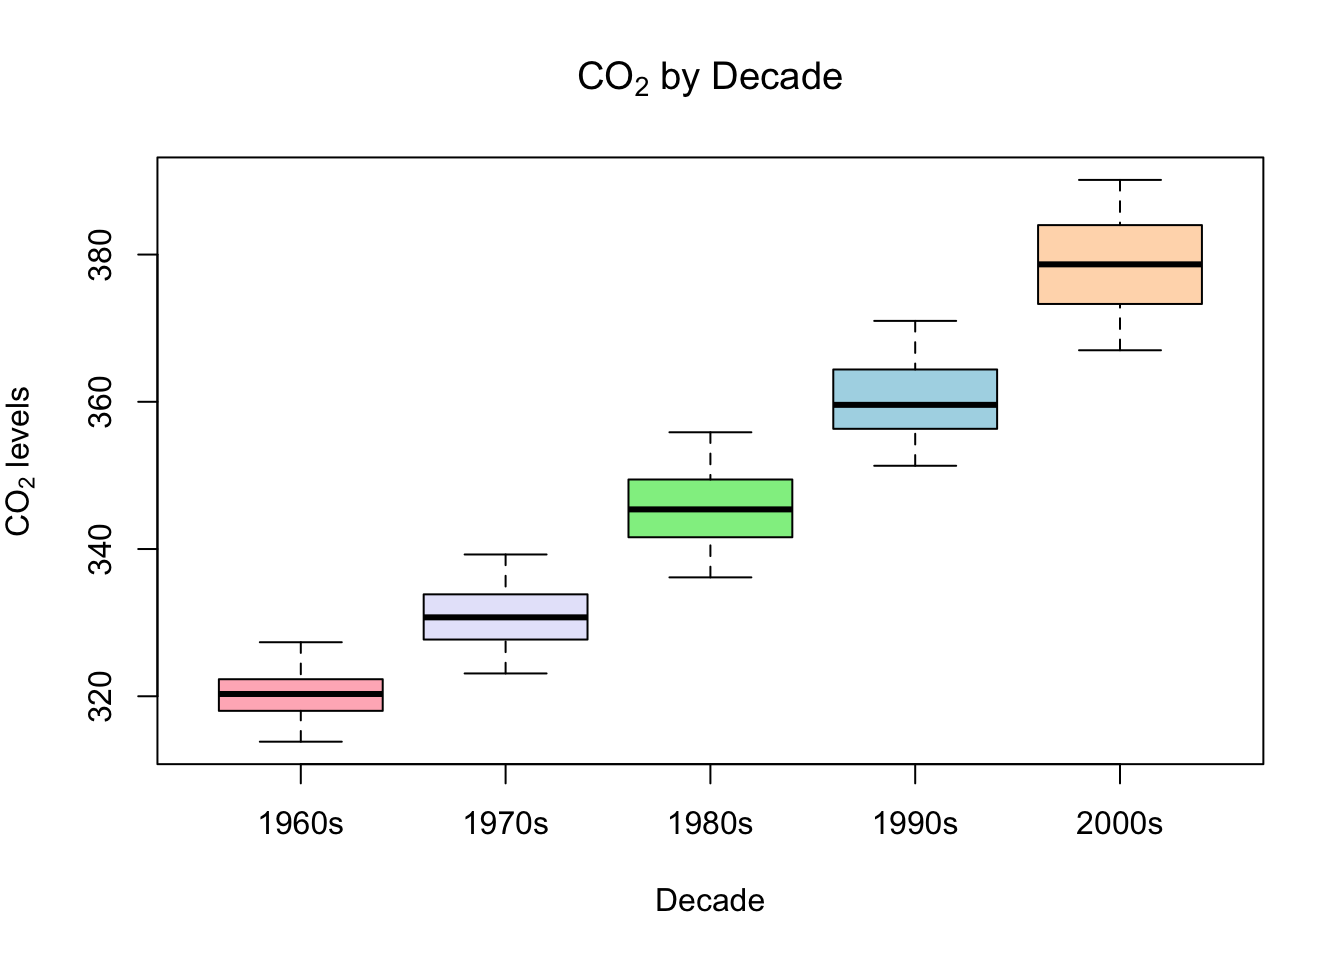
\includegraphics{Project01_files/figure-latex/unnamed-chunk-6-1.pdf}

\begin{verbatim}
## Warning: Removed 20 rows containing non-finite values (stat_boxplot).
\end{verbatim}

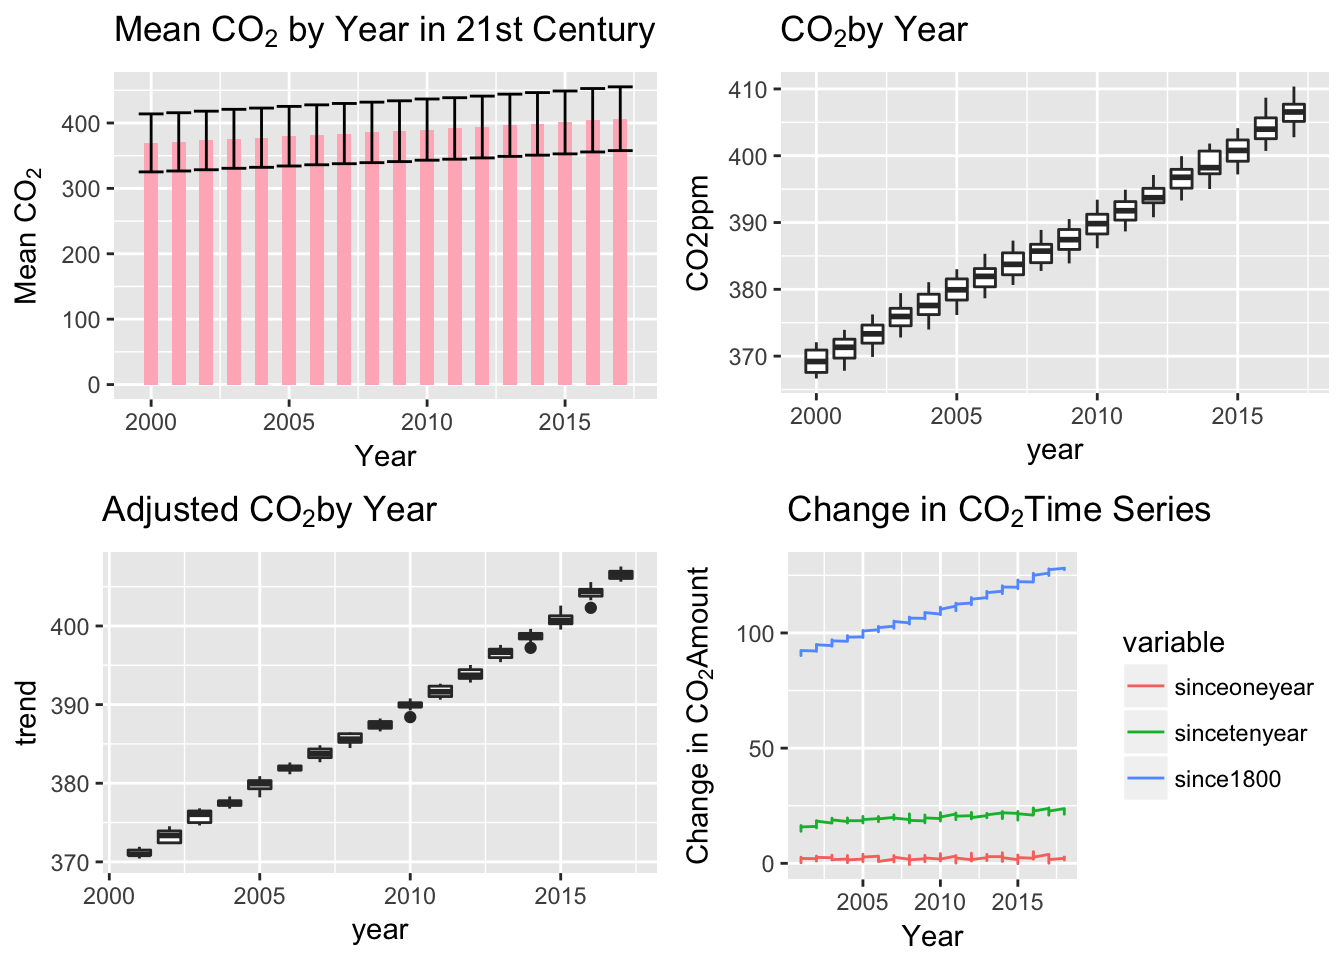
\includegraphics{Project01_files/figure-latex/unnamed-chunk-11-1.pdf}

\subsubsection{QUESTIONS}\label{questions}

\begin{enumerate}
\def\labelenumi{\arabic{enumi})}
\tightlist
\item
  Discuss briefly how these data were collected.
\end{enumerate}

\emph{The data we were given was from Mauna Loa, Hawaii. This is the
complete data from 2014 up until March of 2018. Therefore, the 2018 data
is preliminary. The data was obtained at an altitude of 3,000 m in the
northern subtropics. The data we were given was reported as a dry air
mole fraction defined as the number of molecules of carbon dioxide
divided by the number of all molecules in air and then multiplied by one
million(ppm), this is including CO2 itself after the water vapor has
been removed.}

\begin{enumerate}
\def\labelenumi{\arabic{enumi})}
\setcounter{enumi}{1}
\tightlist
\item
  What trend(s) or patterns over time do you observe in the CO2 graphs?
\end{enumerate}

\emph{All eight of the graphs show a steady increase, or positive
correlation, in CO2 over time. The change in CO2 time series graph
displays that while CO2 is increasing over time, it's not changing
drastically over short periods of time. Therefore sugessting that CO2
levels have been steadily increasing since 1800}

\begin{enumerate}
\def\labelenumi{\arabic{enumi})}
\setcounter{enumi}{2}
\tightlist
\item
  In what way could these analyses be used to support the theory of
  anthropogenic (man-made) climate change? Why are data and graphs such
  as these \emph{evidence} rather than \emph{proof}?
\end{enumerate}

\emph{This data could be used to support the theory of anthropogenic
climate change because every one of the eight graphs show us that the
CO2 level is continuously increasings over time. It is also a fact that
the populaion on Earth is increasing steadily over time. Therefore, we
can suggest that the more people on earth, the more likely the CO2
levels are to rise. This is evidence rather than proof because there are
other factors effecting climate change other than CO2. You can not
predict ahead of time what the other factors will be or what the CO2
levels will be for future years/decades.}


\end{document}
